\chapter{Att observera med SALSA}
Det är viktigt att vara väl förberedd innan du börjar observera med SALSA.
Tiden är inte bara begränsad, på grund av jordens rotation så kan vissa objekt
ses på himlen över Onsala under en kort tid på dagen. Försök att få en bra
förståelse för vad du vill göra med SALSA innan du börjar använda teleskopet.
I detta kapitel så beskriver vi vad du kan observera, hur du styr teleskopet,
och hur du gör en mätning. Vi rekommenderar starkt att du läser hela detta
dokument innan du använder SALSA första gången.

\emph{OBS:} när du är klar med dina observationer, vänligen ställ teleskopet i
viloläge (\verb!Stow! position). Detta görs genom att välja \verb!Stow! i listan
över koordinater i styrprogrammet och sedan trycka på \verb!Track!. I viloläge
så är teleskopen mindre känsliga för starka vindar som kan skada mekaniken. 

\section{Vad kan observeras med SALSA?}
Även om SALSA huvudsakligen har utvecklats för att observera vätgas i vår 
galax Vintergatan så finns det några andra sätt att använda teleskopet. 
I detta avsnitt så beskriver vi de idéer som vi har provat hittils. Fler
projekt kommer att läggas till när vi får tid. 

\subsection{Vintergatan}
De flesta personer som använder SALSA har som mål att detektera radiovågor från 
vätgas i vår galax Vintergatan. Målet är att detektera strålning som sänds ut av
atomärt väte nära frekvensen 1420.4\,MHz. Detta projekt är vad SALSA-hemsidan
och kontrollprogrammet är utvecklade för, och den största delen av dokumentationen
är till för att underlätta dessa mätningar. För en utförlig beskrivning av detta
projekt, se dokumentet \emph{Kartläggning av Vintergatan} som finns att 
ladda ner via SALSA-hemsidan.

\subsection{Solen}
Solen är en stark radiokälla och kan enkelt detekteras med SALSA. Observationer
av solen kan användas för att mäta antennens mottagaregenskaper. Mer information
om detta projekt finns i dokumentet \emph{Antennrespons för SALSA}, som finns
att ladda ner via SALSA-hemsidan. 

\subsection{GNSS satelliter}

Framsteg i rymdvetenskap och utforskning av universum, som inleddes 1960, orsakade att
många satelliter började dyka upp på jordens bana vid höjder från 2000 till 20 000 km.
Sådana konstgjorda föremål används i många olika områden inom vetenskap och teknik, såsom
telekommunikation, meteorologi, miljöövervakning eller navigering. Den senare är realiserad genom
ett så kallat Global Navigation Satellite System (GNSS). SALSA-användare kan upptäcka signaler som emitteras från
GNSS satelliter. Mer information om detta projekt finns i dokumentet
\emph {GNSS signal spectra with SALSA}, tillgänglig på SALSA webbplats.

%\subsection{Cassiopeia A}
%Cassiopeia A is a bright radio source and should be observable
%with SALSA in a way similar to how we observe the Sun. We have not yet
%had the time to verify that we can indeed detect Cas. A, but as soon
%as we do we will provide instructions on the SALSA website. 
%
%\subsection{The Andromeda galaxy}
%The Andromeda galaxy contains a lot of neutral hydrogen, just like the Milky
%Way. In theory we should be able to detect hydrogen emission from Andromeda and
%derive the rotational speed of the galactic disc. However, because the galaxy
%is much further away than the gas clouds in the Milky Way, we will probably
%need to measure for many hours. Unfortunately, SALSA is, for technical reasons,
%not yet capable of doing such long measurements. We aim to improve the system
%in the future to make it possible to detect Andromeda, and when we have
%confirmed that it works we will provide a set of instructions on the SALSA
%website.

\section{När kan SALSA se ett visst objekt?}
Alla himmelska objekt kan inte ses från Onsala, vissa kan bara ses över horisonten
under en kort tid varje dag. Innan du observerar så är det bra att förbereda dig
så att du är säker på att du kan observera det du vill under din bokade tid.
Mer information om hur du gör detta finns i Appendix \ref{app:coord}. Notera att
detta appendix även inkluderar en lista över galaktiska koordinater som alltid
är synliga från Onsala. Dessa kan vara bra positioner att börja med för en 
kartläggning av Vintergatan.

Ett annat sätt för att ta reda på vad du kan se med SALSA vid en viss tidpunkt
är genom att installera gratisprogrammet \emph{Stellarium}, som finns att 
ladda ner via http://stellarium.org/. Ställ in att du är i Onsala (eller i 
Kungsbacka, vilket programmet känner till och som är tillräckligt nära Onsala),
och välj datum och tid. Programmet kommer då att förutse hur himlen ser ut. 
Notera att du kan välja att visa koordinataxlar i Stellarium: både galaktiska
och ekvatoriella koordinater finns som val.

\section{Att ansluta till SALSA} 
\label{sect:connect}
SALSA-teleskopen kontrolleras från datorer i Onsala. Om du är på 
observatoriet så kan du logga in på en dator direkt. Men, de flesta observationer
görs genom att fjärrstyra teleskopet via internet. För att kontrollera SALSA
så måste du alltså logga in på en dator i Onsala via internet. Detta har 
testats utan problem på Windows, Mac OS X och Linux så du bör kunna ansluta 
med  vilken dator som helst. Det finns två vanliga sätt att ansluta
till en dator i Onsala:

\begin{itemize}
	\item{\emph{I din webbläsare.} Detta är det vanligaste
			sättet att fjärrstyra ett SALSA-teleskop. Ingen speciell 
			progamvara behövs förutom en uppdaterad webbläsare. Du hittar länkarna
			till inloggningssidorna för teleskopen på sidan \emph{Observe} på 
			SALSA-hemsidan. 

			OBS: Din webbläsare kommer att klaga på att anslutningen inte är 
			tillförlitlig, \emph{untrusted}, eftersom vi inte har n[got
			certifikat för SALSA-datorerna. Vänligen ignorera denna varning
			för att logga in på datorerna. För att göra detta i Firefox, välj 
			\emph{Jag förstår riskerna, Lägg till undantag, Bekräfta undantag
			}. I Safari: klicka \emph{fortsätt}. I Explorer: klicka \emph{fortsätt}.  
			När du är ansluten så kan du starta kontrollprogrammet genom
			att klicka på SALSA-genvägen på det virtuella skrivbordet, eller genom att
			starta en terminal och skriva SALSA. 
		}
\item{\emph{Terminalen.} Om du är van att arbeta i terminalen så kan du 
		logga in via SSH med grafik genom att köra kommandot 
		{\tt ssh -X username@computer}, där computer är antingen vale.oso.chalmers.se eller
		brage.oso.chalmers.se beroende på vad du bokat.  Du kan sedan starta kontrollprogrammet
		genom att köra kommandot {\tt  SALSA}.}
\end{itemize}

\subsection{Att avsluta din session}
När du är har observerat färdigt, vänligen stäng kontrollprogrammet genom
att klicka på \emph{x} i övre högra hörnet av programmet. Stäng sedan din 
anslutning till SALSA-datorn. Om du är uppkopplad i webbläsaren, stäng din 
anslutning genom att stänga det virtuella skrivbordet, t.ex. genom att
klicka på knappen uppe i höger hörn. 
Om du är uppkopplad via SSH i en terminal så kan du stänga din anslutning
genom att köra kommandot {\tt exit}.

\emph{OBS:} när du är klar med dina observationer, vänligen ställ teleskopet i
viloläge (\verb!Stow! position). Detta görs genom att välja \verb!Stow! i listan
över koordinater i styrprogrammet och sedan trycka på \verb!Track!. I viloläge
så är teleskopen mindre känsliga för starka vindar som kan skada mekaniken. 

\subsection{Felsökning}
Har du problem att ansluta till teleskopdatorn? Innan du kontaktar supporten,
vänligen kolla följande tre vanliga fel:
\begin{itemize} 
\item Lösenordet för kontrolldatorn kan vara ett annat än det du använder för 
	att logga in på hemsidan (för att göra bokningar). För att logga in på
	kontrolldatorn så använder du ditt \emph{telescope password} som du hittar
	under \emph{My account} på SALSA-hemsidan.
\item Kontrollera så att du försöker ansluta till rätt dator. Adressen är 
	olika för olika teleskop, men ser liknande ut. Om du till exempel
	har bokat teleskopet \emph{vale}, då ska du ansluta till 
	\emph{vale.oso.chalmers.se}. Om du har bokat teleskopet \emph{brage},
	då ska du ansluta till \emph{brage.oso.chalmers.se}. 
\item Kontrollera så att du har bokat teleskopet vid rätt tidpunkt. Bokningar
	på hemsidan visas i den tidszon som du valt. Du kan kontrollera vad klockan
	är i den tidszon du valt genom att titta på klockan uppe till höger på
	SALSA-hemsidan.  
	\end{itemize}

\section{Kontrollprogrammet för SALSA}
\label{sect-control}
När du är inloggad på en dator så kan du starta kontrollprogrammet
genom att antingen klicka på genvägen \emph{SALSA} på det virtuella
skrivbordet, eller genom att köra kommandot \emph{SALSA} i en terminal.  
Du bör \footnote{Ibland kan det ta över 10 sekunder innan programmet visas,
	ha tålamod. Om du inte ser något fönster, prova igen. Om du inte ser något
	efter 30 sekunder, kontakta supporten enligt instruktionerna på SALSA-hemsidan.} 
	nu se kontrollprogrammet, se Fig. \ref{fig:controlstart}. 
\begin{figure}[ht]
\begin{center}
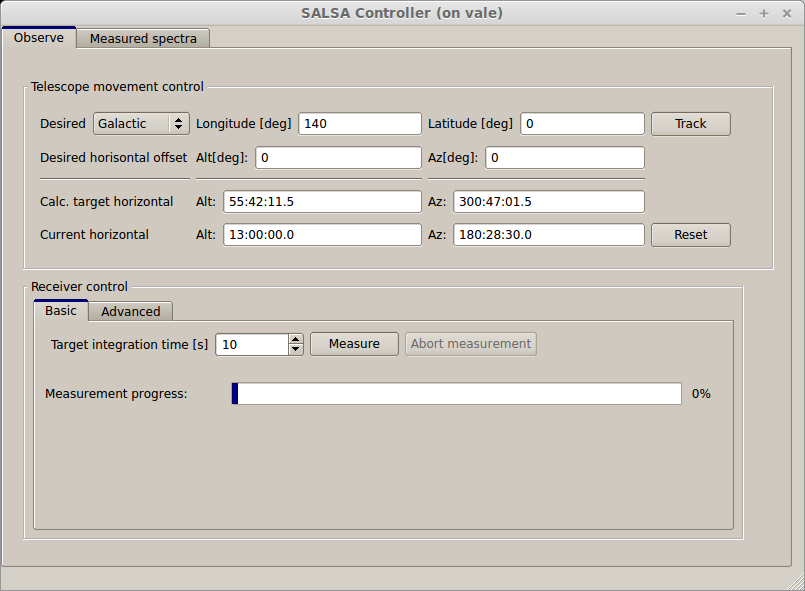
\includegraphics[width=\textwidth]{../figures/Controller_start.png}
\end{center}
\caption{Startläget för kontrollprogrammet.}
\label{fig:controlstart}
\end{figure}
Kontrollprogrammet används för att styra teleskopet och för att göra mätningar. 
Vi börjar med att förklara hur du styr teleskopet, och sedan beskriver vi hur
du gör mätningar. 

\subsection{Movement control: Att peka åt rätt håll}
Kontrollprogramet innehåller en ruta med rubriken \emph{Telescope movement control}. 
Denna ruta innehåller fyra rader av vita fält. Vi beskriver nu syftet med dessa fält
i detalj. 

De första två raderna är till för att användare ska skriva in värden. Den första
raden har etiketten \emph{Desired}. Denna rad måste fyllas i av dig: här anger du
vart du vill att teleskopet ska peka. Du kan välja olika koordinatsystem, men 
galaktiska koordinater är de vanligaste eftersom de är praktiska när du observerar 
vätgas i Vintergatan. Några speciella objekt kan också väljas direkt, till exempel
solen. 

Den andra raden har etiketten \emph{Desired horizontal offset}. Denna rad
används endast i specialfall, t.ex. för att mäta antennresponsen för SALSA. Denna rad
bör lämnas med värdet 0 för de flesta observationer, t.ex. för att observera
vätgas i Vintergatan. 

Raderna tre och fyra visar information, d.v.s. du ska inte skriva in något här.
Den tredje raden har etiketten \emph{Calc. target horizontal}. Denna rad
visar målets lokala (altitude-azimuth) koordinater som de beräknats av kontrollprogrammet
givet de önskade koordinaterna som du skrivit in (inklusive eventuell offset
från rad två). Notera att koordinaterna på rad tre ändras då riktningen
räknas om varje sekund. Dessa omräkningar görs automaiskt av programmet. 

Den fjärde och sista raden visar de nuvarande lokala koordinaterna, d.v.s. 
åt vilket håll antennen pekas just nu. När du säger till antennen att röra sig, se nedan,
så kommer den att röra sig tills de nuvarande koordinaterna på rad fyra
kommer så nära som möjligt den beräknade positionen på rad tre. 

\subsubsection{Tracking}
Tracking betyder att följa eller \emph{tracka} ett specifikt objekt
eller koordinat på himlen. Det innebär att teleskopet beböver röra sig för att
korrigera för jordens rotation (ungefär 0.25$^\circ$ per minut). När du valt
ett önskat mål, klicka på knappen {\tt Track}. Teleskopet börjar nu röra sig, se
Fig. \ref{fig:controlmove}, och kommer att fortsätta att beräkna och följa ditt mål
på himlen tills du säger åt det att sluta genom att klicka på knappen {\tt Stop}.  
Glöm inte att titta på webkameran på SALSA-hemsidan för att se att teleskopet rör sig. 
När du når ditt mål så kommer du troligen inte att se de små korrigeringarna, 
som behövs för att följa målet på himlen, med ögat. Men, om du tittar noga
så kommer du att se att värdena i rad fyra, \emph{Current} coordinates, kommer
att ändra sig lite över tid för att följa en ändring i den beräknade positionen.
Notera att det kan ta upp till några minuter för teleskopet att nå din önskade 
position om du började långt bort på himlen. Att mäta under tiden du rör dig
ger bara nonsens, du måste vänta tills teleskopet har kommit fram till rätt
riktning. 
\begin{figure}[ht]
\begin{center}
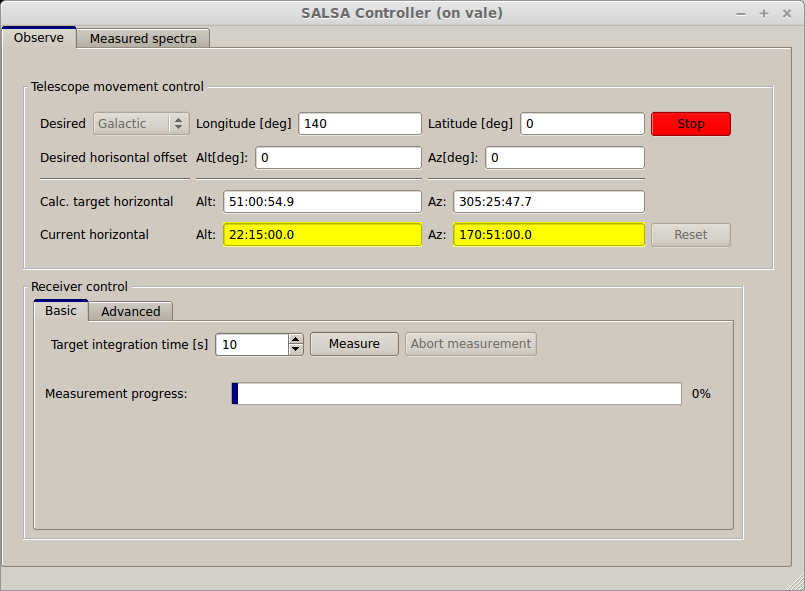
\includegraphics[width=\textwidth]{../figures/Controller_move.png}
\end{center}
\caption{Så här ser kontrollprogrammet ut när teleskopet rör sig.}
\label{fig:controlmove}
\end{figure}

\subsubsection{Hur noggrannt är SALSA?}
Teleskopet har en noggrannhet på 0.5$^\circ$ givet dess mekaniska konstruktion.
Detta är dock mycket mindre än vinkelstorleken på antennens \emph{huvudlob}, d.v.s.
det område på himlen där antennen fångar upp strålning. Huvudloben för SALSA
har uppmätts till ca 5.4$^\circ$ vid frekvensen 1420\,MHz.  Vänligen vänta tills
teleskopet är inom 1$^\circ$ från ditt önskade mål innan du gör en mätning. 
Kontrollprogrammet kommer att visa detta genom att ändra bakgrundsfärgen
på raden \emph{Current} coordinates från gul (vilket innebär att teleskopet
inte är framme ännu, se Fig. ref{fig:controlmove}) till vit (vilket innebär att
teleskopet är redo att mäta). Mer information om noggrannhet hittar du i
kapitel \ref{chap:tech}.

\subsubsection{Mät endast ovanför 15$^\circ$ altitud}
Teleskopet kommer att vägra att röra sig om du försöker få det att peka
åt ett håll som det inte kan, och programmet kommer att tala om för dig
vilka värden som är tillåtna. Du kan alltså inte göra sönder teleskopet genom
att peka åt fel håll. Men, även om teleskopet kan peka ända ner mot horisonten så
är det klokt att bara mäta en bit över horisonten för att undvika störande
radiostrålning från marken. Som en tumregel, observera endast om ditt mål
är mer än 15$^\circ$ över horisonten. 

\subsection{Receiver control: Att göra en mätning}
När teleskopet har nått din önskade riktning så är du redo att göra en mätning. 
Det är viktigt att fortsätta att tracka under tiden du mäter, så klicka inte på 
stop-knappen förrän din mätning är klar. Innan du startar en mätning så
måste du bestämma hur länge du vill mäta. En längre tid ger en tydligare signal. 
Tiden du mäter kallas \emph{integrationstid} och du anger detta i rutan med titeln
\emph{Receiver control} i mitten av programfönstret. Vanligtvis så fås ett bra spektrum
av väte efter 20 sekunder. Efter att du skrivit in integrationstiden, klicka på 
{\tt Measure}. Du kommer nu att se en förloppsmätare som ökar från vänster
till höger i nedre delen av programfönstret, se Fig. \ref{fig:controlmeasure}.
\begin{figure}[ht]
\begin{center}
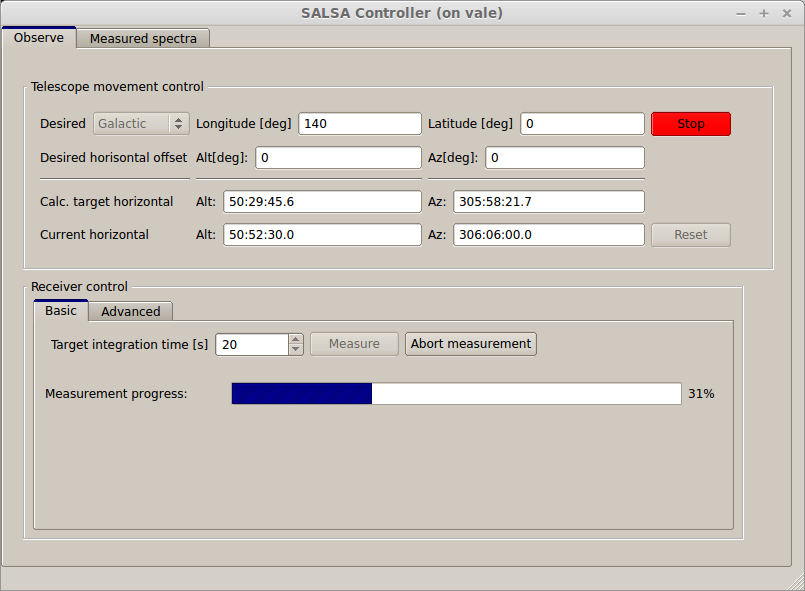
\includegraphics[width=\textwidth]{../figures/Controller_measure.png}
\end{center}
\caption{Kontrollprogrammet när en mätning pågår.}
\label{fig:controlmeasure}
\end{figure}

{\bf Obs.:} Teleskopet kommer, utan att du behöver göra något, att dela den tid
som du anger i rutan \emph{Integration time} i två delar. Detta eftersom
teleskopet, förutom att mäta på ditt mål (signalen du vill ha), också behöver
mäta på sig självt (hur mottagaren stör signalen). Teleskopet gör detta genom
att byta mätfrekvens bort från väte när det mäter på sig självt. Avancerade
möjligheter att styra denna switchning finns under fliken \emph{Advanced}, men
rör inte dessa värden utan att du vet vad du gör. För vanliga användare så
behöver du endast välja integrationstid under \emph{Basic}. 

\subsection{Mätresultat}
\label{sect:inspect}
När en mätning är färdig så lagras spektrumet tillfälligt i kontrollprogrammet. 
För att titta på ditt spektrum, klicka på fliken \emph{Measured spectra} i 
övre delen av programfönstret. Du ser nu ett fönster liknande Fig.  
\ref{fig:controlspectra}. På vänstersidan visas en lista över alla spektra som du
tagit i denna session (sedan du startade programmet). På högersidan visas det spektrum
som är markerat i listan. Denna figur är användbar för en snabb analys av din mätning. 
Du kan zooma genom att använda knapparna under figuren, och om du håller muspekaren
över figuren så visas värdet där du har markören som två tal under figuren. 
\begin{figure}[ht]
\begin{center}
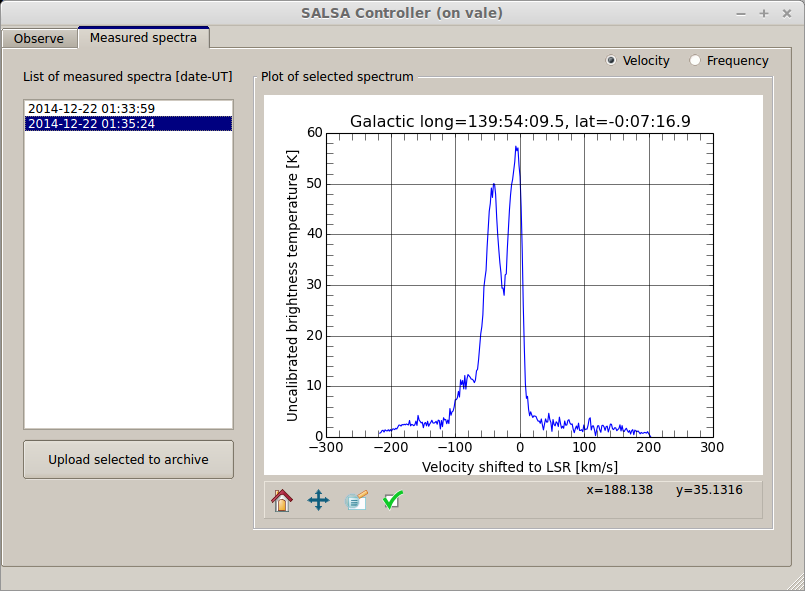
\includegraphics[width=\textwidth]{../figures/Controller_spectra.png}
\end{center}
\caption{Fliken \emph{Measured spectra} i kontrollprogrammet. Till vänster
	visas en lista över alla mätningar som gjorts i denna session. Till höger 
	visas det spektrum som är markerat i listan. Du kan välja ett annat spektrum
	genom att klicka i listan. Nere till vänster finns en knapp för att spara
	det markerade spektrumet genom att ladda upp det till webarkivet. 
}
\label{fig:controlspectra}
\end{figure}
Även om detta är det enklaste sättet att få ut information från din mätning,
så kanske det inte är det mest praktiska. Kanske vill du istället använda din tid
med SALSA till att göra observationer, och sedan göra en noggrann analys av dina
mätningar i efterhand. Då måste du spara din data. I nedre vänsta hörnet finns en 
knapp som du kan använda för att spara det markerade spektrumet till webarkivet.
Efter att du sparat en mätning så kan du hämta den när som helst via SALSA-hemsidan,
se avsnitt \ref{sect:archive}. Datan bör finnas i arkivet någon sekund
efter att du tryck på Upload-knappen, så kolla gärna att din data verkligen 
har laddats upp innan du avslutar kontrollprogrammet. Notera att om du inte 
laddar upp dina mätningar så kommer de att tas bort när du stänger programmet.
\subsubsection{LSR-korrigering}
Skiftet av frekvens som man mäter med SALSA är resultatet av
en hastighetsskillnad mellan teleskopet (observatören) och målet (källan)
längs synfältet. Som standard korrigeras i SALSA den beräknade radiella hastigheten och den uppmätt frekvensen
för observatörens rörelse och uttryckt med avseende på Local-Standard-of-Rest (LSR)
ram. Denna korrigering betraktar två huvudeffekter: solens rörelseförhållande
till LSR och jordens orbitalrörelse i förhållande till solen. LSR-korrigering kan inaktiveras på fliken \emph {Advanced}
om man inte vill använda det här alternativet.
\subsubsection{RFI-borttagning}
Som standard används medianfiltrering i SALSA för att filtrera bort eventuell radiofrekvensinterferens (RFI)
närvaro i den inspelade signalen. Tanken med detta filter är att gå igenom signalvärdet och
ersätta varje värde med medianen av närliggande värden. Det är viktigt att identifiera vilken RFI som direkt
påverkar de erhållna resultaten (Fig.~\ref{fig:RFIremoval}). RFI-borttagning kan dock inaktiveras
fliken \emph {Advanced}, om man inte vill använda det här alternativet.
\begin{figure}[ht]
\begin{center}
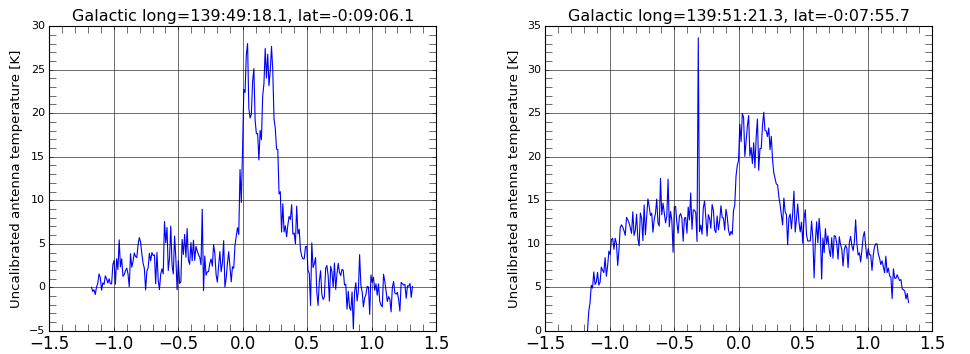
\includegraphics[width=\textwidth]{../figures/RFIremoval.png}
\end{center}
\caption{
RFI-borttagning i SALSA. Spektrat på vänster sida erhölls med standardinställningar där RFI filtreras bort.
Det andra spektrat är ett resultat av en efterföljande mätning där alternativet RFI-borttagning avaktiverats. 
Man kan identifiera en smal och stark topp som är resultat av störningar som genereras av en extern radiokälla.}
\label{fig:RFIremoval}
\end{figure}
\section{Att analysera data från webarkivet}
\label{sect:archiveprocess}
Som beskrivits i föregående avsnitt så kan du inspektera din data direkt i
kontrollprogramet. Detta är det enklaste sättet att få ut information
från dina mätningar, men i vissa fall kanske du vill göra en mer noggrann analys
utan att boka tid med SALSA. I detta avsnitt så beskriver vi hur du öppnar
de olika dataformat som går att hämta från webarkivet och vilken mjukvara
du kan använda för att analysera dina mätningar.

\subsection{PNG: Bilder}
PNG-formatet är en bild av spektrumet, precis som det såg ut i kontrollprogrammet
när du klickade på knappen Upload. Detta är användbart för en snabbtitt på din data,
men är inte lika exakt som att inspektera datan direkt i kontrollprogrammet
eftersom du inte kan få exakta värden från grafen på ett enkelt sätt. 
Men, i många fall kan PNG-bilden vara bra nog för att en grov uppskattning
av t.ex. vilka hastighetskomponenter som ingår i ditt spektrum. En mer
noggrann analys av din data kräver dock tillgång till rådatan. Denna 
kan du hämta som TXT eller FITS, se nedan. 


\subsection{FITS: Ett vanligt format för astronomidata}
En FITS-fil\footnote{Flexible Image Transport System (FITS) format.  En FITS-fil
	innehåller två delar: en header följd av en binär del med datan. Den binära
	tabellen kan förstås och visas med FITS-läsande mjukvara, t.ex. med MATLAB - se
	SALSA-hemsidan. } är ett vanligt format inom astronomi. Detta format
	erbjuder mest funktionalitet och extrainformation. Det finns två vanliga sätt att
	öppna FITS-filer från SALSA:

\begin{itemize}
	\item \textbf{SalsaJ} utvecklades inom projektet EU-HOU och kan användas 
		för att öppna FITS-filer från SALSA.
		SalsaJ är gratis och kräver inga kunskaper om programmering. Programmet SalsaJ och utförliga instruktioner för hur du öppnar FITS-filer finns
		på SALSA-hemsidan {\url{http://vale.oso.chalmers.se/salsa/software}}.
	\item \textbf{SalsaSpectrum} SalsaSpectrum är ett verktyg, skrivet i det
		populära programspråket MATLAB, som kan användas för att visa och
		analysera data från SALSA. För användare som är vana vid MATLAB så är
		detta troligen den bästa lösningen eftersom det både finns möjligheter
		att göra figurer och skriva egna program. Med detta verktyg så är det
		möjligt att analysera många spektra på en gång och lätt att visa
		resultaten.  SalsaSpektrum-verktyget finns att hämta via
		SALSA-hemsidan, och där finns också utförlig dokumentation som
		beskriver hur verktyget kan användas. Vänligen notera att MATLAB kräver
		inte är gratis utan kräver en licens för att kunna användas -
		Observatoriet kan inte erbjuda licenser för MATLAB.
\end{itemize}

\subsection{TXT: Textfiler}
TXT-formatet innehåller ditt spektrum som ren text, d.v.s. som en lista av
hastigheter och intensiteter. Detta är ett enkelt format och det går att använda 
tillsammans med PNG-filerna för att få bra uppskattningar av hastigheter för de olika
topparna i spektrat. Titta först i PNG-bilden för att få en grov uppskattning om var topparna är.
Läs sedan av de exakta värdena i TXT-filen. 
Om du kan programmera så kan du också skriva egen
kod för att visa datan i TXT-filerna i ditt favoritspråk. 

\subsubsection{Python}
Om du är bekant med programspråket Python så kan du läsa FITS-filer genom att
använda biblioteket \emph{astropy.io.fits}. Var dock noga med att kontroller
att du läser in eventuell VLSR-korrektion och referenspixlar på rätt sätt. Du
kan jämföra med resultatet i TXT och PNG-filerna.  Du kan också läsa
TXT-filerna direkt och plotta dem med python.  Om du vill analysera många FITS
filer med python så kanske du kan få användning för de skript som Michael
Olberg gjort för SALSA, de finns tillgängliga här:
https://github.com/molberg/salsa.

\subsection{R}
Om du är bekant med programspråket R så kan du läsa in FITS filerna med R. 
Här kanske du kan få användning för skript som gjorts av Michael Olberg, 
som du hittar på https://github.com/molberg/salsa.
